% Chapter 1

\chapter{Building a many electron model} % Main chapter title

\label{cha:many} % For referencing the chapter elsewhere, use \ref{Chapter1} 

\lhead{Chapter 2. \emph{Building a many electron model}} % This is for the header on each page - perhaps a shortened title

%----------------------------------------------------------------------------------------

\section{Schr\"odinger equation for a one-electron system}\label{sec:TISE}
Throughout this work, we are going to require an accurate description of our system to simulate various processes. In order to achieve this, we must consider systems at the microscopic scale that obey Quantum Mechanics. Therefore, for a one-electron system, the wavefunctions $\psi_n(\boldsymbol{r},t)$ represent the eigenstates and $H$ describes the total energy operator for a particular problem. The corresponding Schr\"{o}dinger equation is given by,
	\begin{equation}\label{eq:many_TDSE}
	H\psi_n(\boldsymbol{r},t)=i\hbar\frac{\partial}{\partial t}\psi_n(\boldsymbol{r},t),
	\end{equation}
where $\boldsymbol{r}$ denotes the ensemble of spatial coordinates. At this stage we leave the Hamiltonian operator undefined as we will discuss this in greater detail during the analysis in Section \ref{sec:theham}.

The aim of this project is to obtain stationary states, where the system is independent with respect to the time component of $\psi_n(\boldsymbol{r},t)$, i.e. the state is unchanged for every value of $t$, $\psi_n(\boldsymbol{r},t) =\psi_n(\boldsymbol{r})$. Equation (\ref{eq:many_TDSE}) is simple to solve for the hydrogen atom or hydrogenic ions, i.e. a nucleus with one electron orbiting, but becomes complicated when expanding to include many electrons. Generally the time dependent component can be separated out as we obtain identical results when considering a wavepacket with evolution time $t$. We assume here the method of separation of variables to solve (\ref{eq:many_TDSE}) by rewriting,
	\begin{equation}\label{eq:many_SOV}
	\psi_n(\boldsymbol{r},t)=\psi_n(\boldsymbol{r})\phi_n(t).
	\end{equation}
Upon direct substitution of (\ref{eq:many_SOV}) into (\ref{eq:many_TDSE}) and selecting the separation constant as $E_n$, then the Hamiltonian, $H$ has a time independent potential energy operator $V(r)$. It is possible to determine the stationary states of this problem by considering
	\begin{equation}\label{eq:many_TDwave}
	\psi_n(\boldsymbol{r},t)=e^{-iE_nt/\hbar}\psi_n(\boldsymbol{r}).
	\end{equation}
We can then arrive at the desired result,
	\begin{equation}\label{eq:many_TISE}
	H\psi_n(\boldsymbol{r})=E_n\psi_n(\boldsymbol{r}).
	\end{equation}
This is known as the time-independent Schr\"{o}dinger equation (TISE). This eigenvalue equation has eigenvector solutions of $\psi_n(\boldsymbol{r})$ with corresponding eigenvalues $E_n$ for each state with index $n$.

The solution of this equation is simple for one-electron systems as we have mentioned, and analytical solutions exist and are readily obtainable. The solution can be determined by a further separation of variables into a set of radial ($r$), and spherical ($\theta, \phi$) coordinates,
	\begin{equation}\label{eq:many_fullwave}
	\begin{split}
	\psi_{nlm_l}(\boldsymbol{r}) =& ~R_{nl}(r)\Theta_{l}(\theta)\Phi_{m_l}(\phi)=R_{nl}(r)Y_{lm_l}(\theta,\phi)\\
	\psi_{nlm_lm_s}(x) =& ~\psi_{nlm_lm_s}(\boldsymbol{r})\chi_{s,m_s}
	\end{split}
	\end{equation}
The wavefunction depends on a set of quantum numbers, $n$, $l$, $m_l$, and $m_s$ which will become clearer in the following Sections when we look at a particular energy operator $H$ (subscripts on the quantum numbers are neglected as we are considering only one electron). Throughout this work, $x$ represents the spatial and spin coordinates collectively, and $\boldsymbol{r}$ is the three dimensional spatial component. Since this spherical coordinate system has no dependence on the electron spin, then the introduction of the spin function $\chi_{s,m_s}$ still results in $\psi_{nlm_lm_s}(x)$ being a solution to equation (\ref{eq:many_TISE}), and the single electron spin is necessarily $s=1/2$. We combine the $\Theta_l(\theta)$ and $\Phi_{m_l}(\phi)$ components to construct the well known Spherical Harmonics, $Y_{lm_l}(\theta,\phi)$, and these functions are easily calculated. Therefore the problem is reduced substantially to solving for the radial component of the wavefunction, $R_{nl}(r)$.

\section{The Hamiltonian for a many electron system}\label{sec:theham}
At this point we have reduced the problem to a time-independent one, and we now have a definition for the form of the single particle wavefunction in equation (\ref{eq:many_fullwave}). What is missing now is the Hamiltonian operator that we had left undefined in equations (\ref{eq:many_TDSE}) and (\ref{eq:many_TISE}). The Hamiltonian is a representation of the total energy in some system which can be constructed from its kinetic and potential energy, written below as,
	\begin{equation}\label{eq:many_TV1V2}
	H=T+V_i=T+V_1 + V_2
	\end{equation}
where $T$ is the kinetic energy operator, and $V_1$ and $V_2$ are two potential energy operators. Once we define appropriate forms for the kinetic and potential energy, we are then in a position to determine the radial contribution of $R_{nl}(r)$.

We can think of a simplistic model for an atomic system containing a few negatively charged electrons surrounding a positive nucleus. This is advantageous in understanding the concepts that are implemented here for the construction of larger multi-electron systems. We must therefore consider the effects of three contributions to the total energy, namely the kinetic energy $\{1\}$ of the electrons, the Coulomb interaction between each orbiting electron and positive nucleus $\{2\}$ and finally, the repulsion that each of the electrons feel from one another $\{3\}$. Obviously in number $\{3\}$, the electron-electron repulsion contribution can be neglected completely for one-electron systems.

In order to proceed, we assume that the nucleus is infinitely heavy (a point mass) comparable to the mass of the remaining electrons. To generalize further, we consider this multi-electron system to have a total of $N$-electrons and a nuclear charge denoted by $Z$. The total kinetic energy operator can be written as
	\begin{equation}\label{eq:many_T}
	T=\sum_{i=1}^N-\frac{1}{2}\nabla_i^2.
	\end{equation}
Therefore this total is just the summation over each individual electron kinetic energy. It follows that the Laplacian operator should also be written in spherical polar coordinates to maintain consistency. Next we consider the interaction of the $i^{th}$ electron with the infinitely heavy nuclear attraction. This potential scales as one over the radial separation between the two particles
	\begin{equation}\label{eq:many_V1}
	V_1=\sum_{i=1}^N\Big(-\frac{Z}{r_i}\Big),
	\end{equation}
where $r_i$ is the electron radius from the nucleus and the summation is over all the electrons again. And finally, the second Coulomb interaction which is that between each pair of electrons is given by
	\begin{equation}\label{eq:many_V2}
	V_2(\boldsymbol{r})=\sum_{i<j}^N\frac{1}{r_{ij}},
	\end{equation}
where $r_{ij} = | \boldsymbol{r}_i - \boldsymbol{r}_j |$. This distance between pairs of electrons can be expanded in terms of spherical harmonics as,
\begin{equation}\label{eq:many_rijspher}
\frac{1}{r_{ij}} = 4\pi\sum_{k}\sum_{k'}(2k+1)^{-1}Y_{kk'}^*(\boldsymbol{\hat{r}}_i)Y_{kk'}(\boldsymbol{\hat{r}}_j)(r_i, r_j)^{k}_{\rm min}(r_i, r_j)^{-(k+1)}_{\rm max}
\end{equation}
and the summation is over all $l$ (index $k$) and $m_l$ (index $k'$) values. It turns out that in equation (\ref{eq:many_TV1V2}), $T+V_1$ is just a summation of one-electron Hamiltonians, and $V_2$ is the interaction between the electrons, i.e. two body effects. In total, the non-relativistic Hamiltonian is therefore the sum of the three equations (\ref{eq:many_T}), (\ref{eq:many_V1}), and (\ref{eq:many_V2}) and then by substituting into equation (\ref{eq:many_TV1V2}) to obtain,
	\begin{equation}\label{eq:many_ham}
	H^N_{{\rm NR}}=\sum_{i=1}^N\Big(-\frac{1}{2}\nabla_i^2-\frac{Z}{r_i}\Big)+\sum_{i<j}^N\frac{1}{r_{ij}}.
	\end{equation}
Upon substitution of this into equation (\ref{eq:many_TISE}) and assuming separation of variables, we are finally in a position to be able to solve the equation for a particular system (We have introduced the superscript $N$ to denote an $N$-particle Hamiltonian here, and for the remainder of this thesis). We revert back to a single electron system first, and by rewriting the orbital angular momentum operators in terms of spherical coordinates, we can obtain the following eigenvalue equations,
	\[
	\boldsymbol{l}^2Y_{lm_l}(\theta,\psi)=l(l+1)Y_{lm_l}(\theta,\psi)
	\]
	\[
	l_zY_{lm_l}(\theta,\psi)=m_lY_{lm_l}(\theta,\psi).
	\]
Where $\boldsymbol{l}^2$ is the total angular momentum operator squared and similarly $l_z$ is its $z$-component of that electron. This is where we first define the orbital angular momentum quantum number $l$ and the magnetic quantum number $m_l$, which has an explicit dependence on $l$, namely $-l \le m_l \le +l$. Similarly we have two eigenvalue equations for $\boldsymbol{s}^2$ and $s_z$, 
	\[
	\boldsymbol{s}^2 \chi_{m_s}(s_z)=s(s+1)\chi_{m_s}(s_z)
	\]
	\[
	s_z\chi_{m_s}(s_z)=m_s\chi_{m_s}(s_z)
	\]
Where the total angular momentum for an $N$-electron system is just these individual angular momenta summed over all electrons,
\begin{equation}\label{eq:many_bigLandbigS}
\boldsymbol{L} = \sum_i^N\boldsymbol{l}_i ~~~ {\rm and} ~~~\boldsymbol{S} = \sum_i^N\boldsymbol{s}_i.
\end{equation}
These four operators commute with the single electron Hamiltonian, and therefore $\boldsymbol{L}^2$, $L_z$, $\boldsymbol{S}^2$, and $S_z$ commute with the $N$-electron Hamiltonian in equation (\ref{eq:many_ham}). We can then define the remaining quantum numbers $s = 1/2$ and $m_s = \pm 1/2$. It is useful to mention that the parity operator $\mathcal{P}$ also commutes with $H^N_{{\rm NR}}$ and determines whether the wavefunction is `even' (positive) or `odd' (negative), and for many electrons the corresponding eigenvalues are $(-1)^{\sum l_i}$. 

\section{The Breit-Pauli Hamiltonian}\label{sec:many_bphamiltonian}
The form of equation (\ref{eq:many_ham}) is a good first approximation, but as $Z$ increases, we must account for relativistic effects. This is due to the fact that the inner most electrons feel a much stronger attractive force from the heavier nucleus. Therefore, assuming the importance of relativistic effects, the Breit-Pauli Hamiltonian can be constructed by expanding the Dirac and Breit Hamiltonian operators discussed by \citet{1957qmot.book.....B} in powers of $\alpha^2$ and neglecting higher orders of $\alpha$. We can now separate the relativistic and non-relativistic contributions of the Hamiltonian in the following way,
	\begin{equation}\label{eq:many_hbp}
	H_{\protect\text{BP}}=H_{\protect\text{NR}}+H_{\protect\text{REL}}.
	\end{equation}
$H_{\protect\text{NR}}$ is simply that of equation (\ref{eq:many_ham}), and $H_{\protect\text{REL}}$ is defined by one and two body correction terms, which leads to further splittings of the energy levels defined as
	\begin{equation}\label{eq:many_hrel}
	H_{\protect\text{REL}}=H_{\protect\text{mc}}+H_{\protect\text{D}}+H_{\protect\text{SO}}.
	\end{equation}
In order to keep the calculations (which are still to be discussed in Chapter \ref{cha:rmatrix}) manageable, we will only be concerned with these one-body terms which are defined by,
	\begin{equation}\label{eq:many_bp1}
	H_{\protect\text{mc}}=-\frac{1}{8}\alpha^2\sum_{i=1}^N\nabla_i^4,
	\end{equation}
	\begin{equation}\label{eq:many_bp2}
	H_{\protect\text{D}}=-\frac{1}{8}\alpha^2Z\sum_{i=1}^N\nabla_i^2\frac{1}{r_i},
	\end{equation}
and
	\begin{equation}\label{eq:many_bp3}
	H_{\protect\text{SO}}=\frac{1}{2}\alpha^2\sum_{i=1}^N\frac{\boldsymbol{l}_i\cdot\boldsymbol{s}_i}{r_i^3}.
	\end{equation}
$H_{\protect\text{mc}}$ is the mass correction term, $H_{\protect\text{D}}$ is the Darwin term and finally $H_{\protect\text{SO}}$ is the spin-orbit term which deals with the coupling between the spin and orbital angular momentum of each electron. $\alpha$ is the fine-structure constant and $\boldsymbol{l}_i$ and $\boldsymbol{s}_i$ are the spin and orbital angular momentum of the $i^{\protect\text{th}}$ electron. The two body terms which are detailed by \citet{1978CoPhC..16...19G} can also be included, and they consist of the spin-other orbit, spin-spin, and orbit-orbit couplings, the two body Darwin terms, and spin-spin contact interaction. They can of course be included as an extension to equation (\ref{eq:many_hbp}), but the corrections are cumbersome when we consider scattering calculations, so we do not include these here. The disadvantage of using equation (\ref{eq:many_hbp}) over the non-relativistic approach is that it does not commute with the operators $\boldsymbol{L}^2$, $L_z$, $\boldsymbol{S}^2$, and $S_z$ due to the additional coupling between the orbital and spin momentum of each of the electrons in equation (\ref{eq:many_bp3}). Informally, this means that $\boldsymbol{L}$ and $\boldsymbol{S}$ are referred to as `bad' quantum numbers and we are forced to introduce a new operator that will commute with $H_{{\rm REL}}$. Even for weak spin-orbit interactions, we must consider the summation of the following total angular momentum,
\begin{equation}\label{eq:many_Jcommutation}
\sum_i^N\boldsymbol{j}_i =\boldsymbol{J} = \boldsymbol{L} + \boldsymbol{S}.
\end{equation}
Where $\boldsymbol{L}$ and $\boldsymbol{S}$ are the operators defined in equation (\ref{eq:many_bigLandbigS}), and the single electron operators satisfy similar eigenfunction equations for $\boldsymbol{j}^2$ and $j_z$, and 
\[
\boldsymbol{j}_i = \boldsymbol{l}_i + \boldsymbol{s}_i
\] 
with `good' quantum numbers $j$, and $m_j$. We therefore find that the fine-structure term for the total $N$-electron Hamiltonian commutes with similar eigenfunctions defined by $\boldsymbol{J}^2$ and $J_z$. 

An accurate description of the system is clearly essential, and equation (\ref{eq:many_hrel}) provides a useful energy operator. However, we are not finished yet, and for complex systems we must obtain approximate wavefunction expansions by applying numerical techniques. The following Sections discuss various approaches with the Hamiltonian operators defined so far.
	
\section{Approximate solutions to the Schr\"odinger\\ equation}\label{sec:manyelectron}
Care must be taken to calculate approximate solutions of the wavefunction using numerical methods. In this Section we will detail multiple methods to determine a many-electron wavefunction. The approximations considered here are the central-field approximation and the Hartree-Fock approximation, which is then extended to consider the configuration-interaction method.

\subsection{Central-field approximation and Hartree's method}\label{ssec:har}
We have provided the form of the Hamiltonian operators for semi-relativistic and non-relativistic cases. To describe the following concepts in this Section, we neglect the one-body correction terms. Therefore we will consider $H_{\protect\text{NR}}$ from equation (\ref{eq:many_ham}) for a many electron system that contains $N$-electrons and nuclear charge denoted by $Z$. As we have already discussed, this equation is not easily separable into $N$ total equations due to the electron-electron repulsion term. 

%
% NEED TO MOVE THIS SOMEWHERE ELSE...
%Therefore, the equation that we will be required to work with is that of the TISE (\ref{TISE}) where we now replace $%\psi(\boldsymbol{r})$ by $\psi(q_1,q_2,...,q_N)$. Here, the various $q_i$ denotes both the spatial and spin coordinates of %the $i^{\protect\text{th}}$ electron. This new N-electron wavefunction $\psi(q_1,...q_N)$ is completely antisymmetric %due to the indistinguishability of the electrons. Therefore $\psi$ is invariant under a change of ordinates, e.g. if %$q_1\rightarrow q_2$ and $q_2\rightarrow q_1$.
% END
%

To apply the central-field approximation, we consider an indirect approach to perturbation theory. We also assume that each electron in the system feels an identical potential, which is represented by the attractive potential of the nucleus and the remaining $(N-1)$ electrons. We can safely assume this as we know that each electron feels a combined force of the nuclear attraction and electron-electron repulsion. This means that the potential only depends radially on the distance between the nucleus and the $i^{\protect\text{th}}$ electron, and a consequence of this is that $\sum_{i<j}\frac{1}{r_{ij}}$ must contain a large spherically symmetric part. To simplify things, we think of an average `screening' effect which we denote as $V_{s}(r_i)$ depending only on the radial coordinate.

%
%We consider the $i^{\protect\text{th}}$ electron in which the distance $r_i$ is both small and large from the nucleus compared to the remaining electrons. This provides a good starting point for the many electron system as the intermediate distances for $r_i$ become problematic.
%

We redefine a new Hamiltonian consisting of an unperturbed $(H_1)$ and a perturbed part $(H_2)$,
	\begin{equation}\label{eq:many_hampert}
	H=H_1+H_2
	\end{equation}
where we simply reformulate by setting
\begin{equation}\label{eq:many_cfham}
 H_1 = \sum_{i=1}^N \Big(-\frac{1}{2}\nabla_i^2+ V_s(r_i)\Big)
\end{equation}
and,
\begin{equation}\label{eq:many_H2}
H_2 = \sum_{i<j=1}^N \frac{1}{r_{ij}} -\sum_{i=1}^N\Big( \frac{Z}{r_i} + V_s(r_i)\Big)
\end{equation}


\begin{figure}
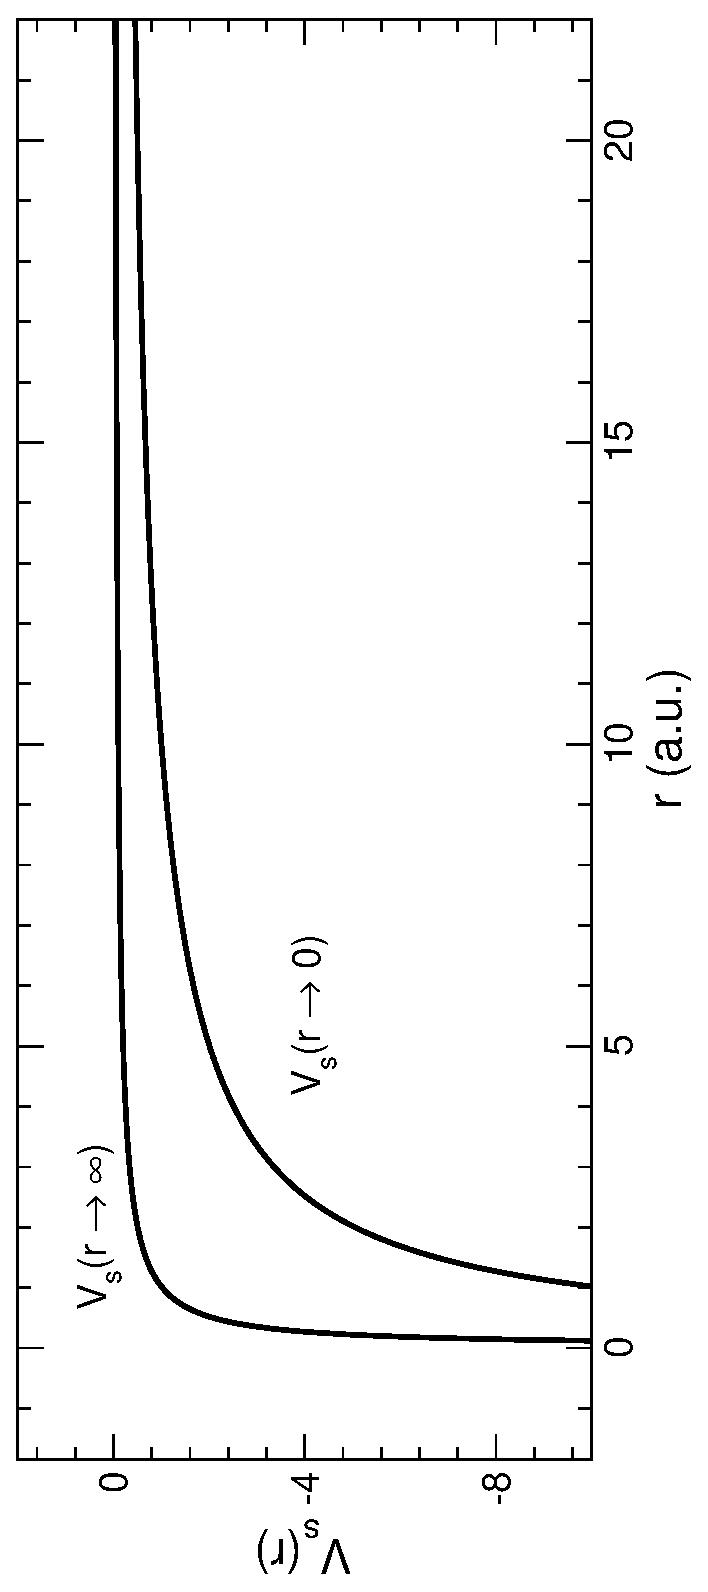
\includegraphics[scale=0.555,angle=-90]{Figures/many_electron/vscreen.eps}
\caption{The right hand sides to the limiting screening potentials defined in equations (\ref{eq:many_vsrzero}) and (\ref{eq:many_vsrinf}) for a test case Ne {\sc i} as a function of the radial distance.  \label{fig:many_vs}}
\end{figure}

Now the major contribution is contained within $H_1$ and the effects of $H_2$ are therefore negligible compared to $H_1$ ($H_2$ << $H_1$). We haven't introduced anything new as the $V_s(r_i)$ will cancel when considering the combined equation (\ref{eq:many_hampert}). This segregation of the Hamiltonian also resembles the form of equation (\ref{eq:many_hbp}), and we can see that the non-relativistic and relativistic contribution represent an unperturbed and perturbed part of the total Hamiltonian respectively. As an initial approximation we disregard the perturbation $H_2$ in equation (\ref{eq:many_H2}) and focus on the central-field Hamiltonian, which is precisely that of (\ref{eq:many_cfham}). At this stage it looks like nothing has changed from our original argument, but now we actually do know the form of $V_s(r_i)$ in its limiting cases, \\
\begin{equation}\label{eq:many_vsrzero}
V_s(r_i \rightarrow 0) = -\frac{Z}{r_i}
\end{equation}
and
\begin{equation}\label{eq:many_vsrinf}
V_s(r_i \rightarrow \infty) = -\frac{Z-N+1}{r_i}     . 
\end{equation}
The right hand sides of these equations can be visualized from Figure \ref{fig:many_vs}, where we sketch both potentials for a neutral case, i.e. $Z=N=10$. The real form of the potential therefore lies somewhere between these two results. Therefore, by considering equation (\ref{eq:many_cfham}), the wavefunction is now separable into a product of $N$, single variable functions for each of the $r_i$.

A similar approach was suggested by Hartree, who had written the total wavefunction for a many-electron problem as the products of the single-electron wavefunctions in equation (\ref{eq:many_fullwave}),
\begin{equation}\label{eq:many_hwave}
\psi(\boldsymbol{r}_1, ..., \boldsymbol{r}_N) = u_1(\boldsymbol{r}_1)u_2(\boldsymbol{r}_2)...u_N(\boldsymbol{r}_N)
\end{equation}
where we have omitted the spin component from the above equation for this analysis and replaced the single-electron wavefunctions by $u_i(\boldsymbol{r}_i)$. The two-body interaction of the electron-electron repulsion can be simplified by assuming the electron moves independently in the field of the remaining electrons, and by spherically averaging this over all angles,
\[
V_i(r_i) = \int V_i(\boldsymbol{r}_i)d\Omega_i = \int \sum_{j\ne i}^{N}\int\frac{|u_j(\boldsymbol{r}_j)|^2}{r_{ij}}  d\boldsymbol{r}_jd\Omega_i.
\]
First we combine the Hamiltonian in equation (\ref{eq:many_ham}) in the approximation of equation (\ref{eq:many_cfham}). Then by considering some wavefunction in the form of equation (\ref{eq:many_hwave}) denoted as Hartree's wavefunction, and upon separation of variables we obtain
	\begin{equation}\label{eq:many_hartree-eq}
	\Big[-\frac{1}{2}\nabla_{i}^2-\frac{Z}{r_i}+V_i(r_i)\Big]u_i(\boldsymbol{r}_i)=E_iu_i(\boldsymbol{r}_i), ~~~~~~~ i=1,...,N
	\end{equation}
where the total energy $E =\sum_i^NE_i$. This particular approach eliminates the complications arising from the electron-electron repulsion and has now become separable into a total of $N$ equations. The functions $u_i(\boldsymbol{r_i})$ are those as defined by equation (\ref{eq:many_fullwave}),
\begin{equation}\label{eq:many_orbitals}
u_{n_il_im_{l_i}m_{s_i}}(\boldsymbol{r}_i) = \frac{1}{r_i}P_{n_il_i}(r_i)Y_{l_im_{l_i}}(\theta_i,\phi_i)
\end{equation}
where we can now express the differential equation from equation (\ref{eq:many_hartree-eq}) in terms of the $P_{n_il_i}(r_i)$ functions, and $R_{n_il_i}(r_i) = \frac{1}{r_i}P_{n_il_i}(r_i)$ has also been introduced. This is useful during the normalization of the radial function and also when solving the differential equations during the numerical integration.

\subsection{Hartree-Fock approximation}\label{ssec:hf}
The Hartree-Fock approximation is based on an independent particle model. The major problem that arises from Hartree's initial assumption is due to the fact that the wavefunction is not antisymmetric in both spin and spatial coordinates in accordance to the interchange of any two electrons. This of course is prohibited due to the effect of the Pauli exclusion principle which is expressed by the following statement,

\protect\textit{``No particles with spin-1/2 may contain identical quantum numbers $n, l, m_l, m_s$ simultaneously.}''

In order to overcome this problem with Hartree's initial wavefunction in equation (\ref{eq:many_hwave}), Fock and Slater proposed a remedy by rewriting $\psi$ in terms of an $N\times N$ dimensional Slater determinant,
	\begin{equation}\label{eq:many_slaterdet}
	\psi(x_1,..,x_N) = \frac{1}{\sqrt{N!}}\left| \begin{array}{cccc}
	u_{\alpha_1}(x_1) & u_{\alpha_2}(x_1) & ... & u_{\alpha_N}(x_1)\\
	u_{\alpha_1}(x_2) & u_{\alpha_2}(x_2) & ... & u_{\alpha_N}(x_2)\\
	\vdots & \vdots & \ddots & \vdots \\
	u_{\alpha_1}(x_N) & u_{\alpha_2}(x_N) & ... & u_{\alpha_N}(x_N) \end{array} \right|.
	\end{equation}
Each $\alpha_i$ denote a set of 4 quantum numbers $\{n_i, l_i, m_{l_i}, m_{s_i}\}$, and $s=1/2$ in accordance with the Pauli exclusion principle. The factor in front of the determinant is to ensure the wavefunction is to be normalized to unity. Without loss of generality, we can assume that the $u_{\beta_i}(\boldsymbol{r})$ are orthonormal to one another, where we have introduced $\beta_i$ to denote the same set of quantum numbers minus the magnetic spin contribution $m_s$. We also relabel $\beta_i \equiv i$ for the equation,
	\begin{equation}\label{eq:many_unorm}
	\Braket{u_i | u_j} = \int u_i^*(\boldsymbol{r})u_j(\boldsymbol{r})d\boldsymbol{r} = \delta_{ij}
	\end{equation}
	where the integral is over all spatial coordinates. Similarly, to account for the magnetic spin term we set $\{m_{s_i}\} \equiv i$, and write
	\begin{equation}\label{eq:many_spinnorm}
	\Braket{\chi_{i} | \chi_{j}} = \sum_{s_z=-1/2}^{+1/2}  \chi_{i}^*(s_z)\chi_{j}(s_z)= \delta_{ij}.
	\end{equation}
The antisymmetric properties arise from the interchange of two rows or two columns, which results in the change of sign of the wavefunction. Also, the wavefunction becomes zero when a set of quantum numbers are equal to each other ($\alpha_i=\alpha_j$).

We can attempt to obtain an optimal Slater Determinant by consideration of the non-relativistic Hamiltonian $H_{\protect\text{NR}}$, from equation (\ref{eq:many_ham}). In the central-field approximation, it was possible to alter the Hamiltonian in such a way to apply perturbation theory. Another approximate method that can be applied whenever it is difficult to find a good description of an unperturbed Hamiltonian is the variational principle. We assume some trial wavefunction with adjustable (variational) parameters and we optimize these parameters until the energy is minimized. The approximate energy functional corresponding to some trial wavefunction $\Phi$ is given by,
	\begin{equation}\label{eq:many_varprinc}
	E_0\leq E[\Phi]= \frac{\Braket{\Phi |H|\Phi}}{\Braket{\Phi |\Phi}}
	\end{equation}
which provides an upper bound to the ground state energy $E_0$. The reason for applying this variational method is to deduce the unknown radial functions, $P_{nl}(r)$.

The minimization procedure is subject to the orthonormality constraints as outlined in equations (\ref{eq:many_unorm}) and (\ref{eq:many_spinnorm}). By taking the trial wavefunction as described in equation (\ref{eq:many_slaterdet}), the functional $E[\psi]$ corresponding to equation (\ref{eq:many_varprinc}) is then made stationary with respect to small variations in the orbitals $u_{\lambda}(x)$ for each $\lambda=\alpha_1, \alpha_2,..., \alpha_N$. By making an infinitesimal change to each of the $u_{\lambda}(x)$ we obtain
	\begin{equation}\label{eq:many_deltaE}
	\delta E-\sum^{\alpha_N}_{\lambda = \alpha_1}\sum^{\alpha_N}_{\mu = \alpha_1}\mathcal{L}_{\lambda\mu}\delta\Braket{u_\mu |u_\lambda}=0,
	\end{equation}
where we have introduced $N^2$ Lagrange multipliers, $\mathcal{L}_{\lambda\mu}$. It is possible to obtain a new diagonal matrix of Lagrange multipliers by performing a unitary transformation on the spin orbitals, $\bar{u}_{\lambda} = \sum_{\mu}U_{\mu\lambda} u_{\mu}$ and therefore $\mathcal{L}_{\lambda\mu} = E_{\lambda}\delta_{\lambda\mu}$, since these Lagrange multipliers form a Hermitian matrix. Assuming that we have selected this unitary transformation from the start, equation (\ref{eq:many_deltaE}) leads to a set of $N$ integro-differential equations, viz, 	
       \begin{equation}\label{eq:many_HF}
	\Big[-\frac{1}{2}\nabla_{i}^2+\mathcal{V}^{(c)}_{\lambda}(x_i)\Big]u^{(c+1)}_\lambda(\boldsymbol{r}_i)=E_\lambda u^{(c+1)}_\lambda(\boldsymbol{r}_i).
	\end{equation}
where $u_{\lambda}^{(c)}(\boldsymbol{r}_i)$ is the spatial part of $u^{(c)}_{\lambda}(x_i)$ at the $c^{\rm th}$ iteration. This has a similar form to that of equation (\ref{eq:many_TISE}) but with a non-local potential $\mathcal{V}^{(c)}(x_i)$ given by,
	\begin{equation}\label{eq:many_HFpot}	
		\begin{split}
	\mathcal{V}^{(c)}_{\lambda}(x_i)=-\frac{Z}{r_i} + & \Bigg[\sum_{\mu}\int u_\mu^*(\boldsymbol{r}_j)\frac{1}{r_{ij}}u_\mu(\boldsymbol{r}_j)d\boldsymbol{r}_j\Bigg]   \\
	- & \Bigg[\delta_{ab}\sum_{\mu}\int u_\mu^*(\boldsymbol{r}_j)\frac{1}{r_{ij}}u_\lambda(\boldsymbol{r}_j)d\boldsymbol{r}_j\Bigg] \frac{u_\mu^{(c)}(\boldsymbol{r}_i)}{u_\lambda^{(c)}(\boldsymbol{r}_i)}.
		\end{split}
	\end{equation}
Now the indices on the Kronecker delta represent the spin quantum numbers, i.e. $a\equiv \{m_{s_a}\}$, and $b\equiv \{m_{s_b}\}$. The equations (\ref{eq:many_HF}) together with the potential in equation (\ref{eq:many_HFpot}) are non-linear, and known as the Hartree-Fock equations. They are solved iteratively at each value for $c > 1$, the first summation in equation (\ref{eq:many_HFpot}) is known as the direct potential, and the second summation accounts for the exchange of electrons and is known as the exchange potential.

\protect{\large{\textit{Self-consistent field method}}}\\
To solve the set of equations (\ref{eq:many_HF}), we briefly outline an iterative procedure known as the self-consistent field method that is applicable in this case. We have already stated that the Hartree-Fock equations (\ref{eq:many_HF}) are not easily solvable, since they amount to a set of integro-differential equations.

The first step in the iterative method starts with an appropriate approximation for the spin-orbitals $u_{\alpha_1}^{(1)}, u_{\alpha_2}^{(1)}, ... ,u_{\alpha_N}^{(1)}$ so that we can then determine $\mathcal{V}^{(1)}$. The integrals are solved for this first iteration and used to determine the set of differential equations in equation (\ref{eq:many_HF}), and therefore solving these equations produces a new set of orbitals, $u_{\alpha_1}^{(2)}, u_{\alpha_2}^{(2)}, ... , u_{\alpha_N}^{(2)}$. The process will terminate when $\mathcal{V}^{(c)}$ is close to $\mathcal{V}^{(c+1)}$ within a pre-specified accuracy, and a similar constraint for the orbitals.

\citet{1974ADNDT..14..177C} represents the radial component of these orbitals by a linear combination of analytical basis functions,
	\begin{equation}\label{eq:many_boundorbs}
	P_{nl}(r)=\sum_{j=1}^kc_{jnl}r^{I_{jnl}}e^{-\eta_{jnl}r}
	\end{equation}
where $c_{jnl}$, $I_{jnl}$ and $\eta_{jnl}$ are coefficients. These are known as Slater-type orbitals (STO's) and describe the general radial form of the wavefunction. The summation grants additional flexibility to their form and the orthonormality conditions from equation (\ref{eq:many_unorm}) also implies that the radial components are orthogonal,
\begin{equation}\label{eq:many_rnlnorm}
\Braket{R_{nl}(r) | R_{\bar{n}\bar{l}}(r)} = \int R_{nl}^*(r)R_{\bar{n}\bar{l}}(r) r^2dr= \int P_{nl}^*(r)P_{\bar{n}\bar{l}}(r) dr =  \delta_{nl,\bar{n}\bar{l}}.
\end{equation}
We will refer to and implement these Hartree-Fock orbitals in future calculations when constructing atomic models. A large tabulation of these are also available in the tables of \citet{1974ADNDT..14..177C}, with details of the calculations therein.

\subsection{The configuration-interaction method}\label{sec:many_ci}
We introduce the configuration-interaction method to account for electron correlation effects, corresponding to a better description of the total wavefunction states. We will therefore investigate how $\Psi_{{\rm HF}}$ can be extended to obtain a better description of these wavefunctions. We begin by considering the angular momentum rules of Russell-Saunders, known as $LS\pi$-coupling outlined in equation (\ref{eq:many_bigLandbigS}).

To account for the electron correlation, we must construct a linear combination of configuration state functions (CSF's). These corresponding atomic state functions (ASF's) then denote some representation of electrons residing in specific orbital shells with quantum numbers $n$ and $l$ that obey the Pauli exclusion principle. The ASF's can be expressed in the following way,
	\begin{equation}\label{eq:many_ciwave}
	\Psi(LS\pi)=\sum_{i=1}^Mc_i\Phi_i(\alpha_iLS\pi)
	\end{equation}
where the CSF's are denoted by $\Phi_i(\alpha_iLS\pi)$, the total wavefunction as $\Psi(LS\pi)$, and $L$, $S$ and $\pi$ being the total orbital and spin angular momentum and the parity of a specific term. These configuration-interaction wavefunctions are typically preferable over the Hartree-Fock description, as $\Psi_{{\rm HF}}$ is often represented by a single CSF. A better approximation of $\Psi(LS\pi)$ will carry an infinite summation, but for practical reasons we terminate with a finite value for $M$. The set of coefficients $\{c_i\}$ are then the weighted contributions from the individual CSF's to the total wavefunction, and $\alpha_i$ represent how the individual electrons $l_i$ and $s_i$ couple together for a total $L$ and $S$. Therefore we require two things; optimized coefficients and CSF's to obtain an accurate total state representation. A similar expression can be written for the fine-structure wavefunction states, $\Psi(J\pi)$ when considering the semi-relativistic corrections of equation (\ref{eq:many_hbp}).\\

\protect{\large{\textit{Optimization of $c_i$'s}}}\\
The first stage is to determine this set of coefficients, $\{c_i\}$. By considering the variational principle in equation (\ref{eq:many_varprinc}) again, we can keep the $\Phi$'s fixed (which we still do not know) while the coefficients constitute the variational parameters. We also perform the minimization subject to the orthonormality of the total $\Psi(LS\pi)$. Assuming $\Psi(LS\pi)$ in equation (\ref{eq:many_ciwave}) as our total wavefunction for a particular state, together with the variational principle, we can obtain the following equation,
\begin{equation}\label{eq:many_optc}
\delta \Big[ \sum_i \sum_j c_ic_j\Braket{\Phi_i | H | \Phi_j} - E_i\Big(\sum_i \sum_j c_ic_j\Braket{\Phi_i | \Phi_j} -1\Big)\Big] = 0.
\end{equation}
Here we have introduced $M$ Lagrange multipliers, labelled as $E_i$. The CSF's constitute an orthonormal set, similarly to the ASF's, and this variational principle reduces equation (\ref{eq:many_optc}) to an eigenvalue problem,
\begin{equation}\label{eq:many_hij}
\sum_j^{M}c_j(\Braket{\Phi_i | H | \Phi_j} - E_i\delta_{ij}) = 0 ~~~ i=1,...,M.
\end{equation}
Therefore, the eigenvector components $\{c_i\}$ also represent the contribution of the diagonalized matrix elements $\Braket{\Phi_i | H | \Phi_j}$ for a particular ASF. This ASF is also categorized by its Lagrange multipliers $E_i$, as they also correspond to their energy eigenvalues.\\

\protect{\large{\textit{Optimization of $\Phi_i$'s}}}\\
We have defined our basis expansion to have a total of $M$ CSF's to describe a particular wavefunction, $\Psi(LS\pi)$. The corresponding set of eigenvalues for a basis set of size $M$ can be easily ordered in the following way,
\begin{equation}\label{eq:many_hyll1}
E_1^{(M)} < ... < E_M^{(M)}.
\end{equation}
Then by including an additional CSF, $\Phi^{(M+1)}$, we can also order the corresponding $E_i^{(M+1)}$ in a similar fashion to equation (\ref{eq:many_hyll1}). The Hylleraas-Undheim theorem states that we can interleave these as follows,
\begin{equation}\label{eq:many_hyll2}
 ... < E_{i-1}^{(M)} < E_i^{(M+1)} < E_i^{(M)}  < E_{i+1}^{(M+1)} < ...
\end{equation}
It is not hard to see from equation (\ref{eq:many_hyll2}) that the inclusion of more CSF's indicates some convergence of the basis set. This is obviously not possible to implement in practice, but it is clear that if $M \rightarrow \infty $, then we obtain an upper bound for the exact energy,
\[
E_i^{(M)} > E_i^{(exact)}
\]
which provides a minimization constraint for all excited states $i$. It should also be mentioned that for the sketched proof above, we have written $E_i$ to represent the $i^{th}$ lowest eigenvalue for this choice of $M$ CSF's.

\section{Transition probabilities}\label{sec:many_transition}
Until now we have been focused on obtaining multiple ways to describe the wavefunctions for as many states as possible. The next step is to consider what happens when some transition between two states takes place. We begin by considering three important mechanisms below.\\

\protect{\large{\textit{Spontaneous emission}}}\\
Suppose that we have a total of $N_j(t)$ atoms at a particular time $t$, where the subscript represents the number in that state $\Ket{j}$. Then the rate of change to some other sate $\Ket{i}$ can be written as,
\[
\frac{dN_j(t)}{dt} = -N_j(t)A_{j\rightarrow i}.
\]
This equation can be extended to consider the total spontaneous emission
\begin{equation}\label{eq:many_spontaneous}
\frac{d N_j(t)}{dt} = - N_j(t)\sum_i^{j-1}A_{j \rightarrow i},
\end{equation}
which is solvable for $N_j(t)$. The summation in equation (\ref{eq:many_spontaneous}) allows for decay to any levels that lie energetically below the current occupancy. Due to the conservation of energy, the spontaneous emission from an upper state $(j)$ to a lower state $(i)$ simply means that the system loses energy in the form of a photon $h\nu_{ji}$, so the change in energy is therefore subject to $h\nu_{ji} = E_j - E_i$. The subscripts on $\nu$ will often be omitted but are included for clarity here. Another useful property is to consider the mean lifetime of $\Ket{j}$ before it radiatively decays, and is defined as
\[
\tau_j = \frac{1}{\sum_i^{j-1}A_{j \rightarrow i}}
\]
which is just the mean time it takes for some state $\Ket{j}$ to decay (i.e. lose energy) to any of the remaining $(j-1)$ states that lie energetically below it.\\

\protect{\large{\textit{Stimulated emission $\&$ absorption}}}\\
We must also account for external influences acting on the system that can alter the internal energy. The first that we describe is known as stimulated emission, $B_{j \rightarrow i}$, which resembles the process of spontaneous emission. The difference is that the system is provided with some form of energy, but enough energy is still lost for a decay to a lower level to occur. The second mechanism is stimulated absorption, where the system gains an amount of energy and therefore excited states can be reached, and is written similarly as $B_{i \rightarrow j}$. This can occur due to the presence of an isotropic, external radiation field, and we assume that the energy per unit volume of this field is $\rho(\nu)d\sigma$. Therefore we can summarize the rate that atoms in state $\Ket{j}$ are stimulated to a lower level $\Ket{i}$ is described by the following,
\begin{equation}\label{eq:many_semission}
\frac{d N_j(t)}{dt} = - B_{j \rightarrow i}N_j(t)\rho(\nu_{ji}).
\end{equation}
Then the absorption of atoms in a state $\Ket{i}$ to a higher state $\Ket{j}$ are given by the rate,
\begin{equation}\label{eq:many_sabsorption}
\frac{d N_i(t)}{dt} = - B_{i \rightarrow j}N_i(t)\rho(\nu_{ji}).
\end{equation}
By assuming detailed balance, we must have equality between the rate of absorption and stimulated plus spontaneous emission between two states. This allows us to relate the following quantities in equations (\ref{eq:many_spontaneous}), (\ref{eq:many_semission}) and (\ref{eq:many_sabsorption}) as
\begin{equation}\label{eq:many_AwithBB}
N_j(t)(A_{j \rightarrow i}+B_{j \rightarrow i}\rho(\nu_{ji})) = B_{i \rightarrow j}N_i(t)\rho(\nu_{ji}).
\end{equation}
By applying Plank's law for $\rho(\nu_{ji})$, and Boltzmann's equation for level populations, we find that
\begin{equation}\label{eq:many_boltz}
\frac{N_j(t)}{N_i(t)} = \frac{g_j}{g_i}e^{-(E_j-E_i)/kT},
\end{equation}
where $k$ is the Boltzmann constant and $T$ is the temperature, it is now possible to rearrange equation (\ref{eq:many_AwithBB}). The stimulated coefficients can also be related to the absorption coefficients by a ratio of statistical weights,
\begin{equation}\label{eq:many_BtoB}
B_{j \rightarrow i} = \frac{g_i}{g_j}B_{i \rightarrow j}.
\end{equation}
We have introduced the statistical weight of a particular level the first time, and we will use this notation throughout the thesis. We define,
\begin{equation}\label{eq:many_statweight}
g_k = \left\{
  \begin{array}{lr}
     (2L_k+1)(2S_k+1)\\
    (2J_k+1)
  \end{array}
\right.
\end{equation}
as be the weight of some state $\Ket{k}$. This weighting is due to the degeneracy in $L$, $S$, and $J$, for example $-L\leq M_L\leq L$. 

\section{Oscillator strengths}\label{sec:many_oscillator}
Another useful quantity is known as the oscillator strength, which measures the strength of absorption between a lower state $\Ket{i}$ to a high lying state $\Ket{j}$. This newly defined oscillator strength can be rewritten in terms of the absorption coefficient,
\begin{equation}\label{eq:many_fwithb}
f_{i\rightarrow j} = \frac{\mu}{\pi e^2}h\nu_{ji}B_{i\rightarrow j},
\end{equation}
where $\mu$ and $e$ are the reduced mass and electronic charge of the electron respectively. In atomic units these quantities are set to unity. This allows us to obtain a relationship between the emission oscillator strength and absorption oscillator strength by substituting equation (\ref{eq:many_BtoB}) into equation (\ref{eq:many_fwithb}),
\[
f_{i\rightarrow j} = -\frac{g_j}{g_i}f_{j\rightarrow i}.
\]
Also from equation (\ref{eq:many_fwithb}), the relationship with the absorption coefficient $B_{i \rightarrow j}$ provides another useful relationship between the transition probability and oscillator strength by applying equation (\ref{eq:many_AwithBB}) and equation (\ref{eq:many_BtoB}) to obtain
\begin{equation}\label{eq:many_fijandaij}
f_{i\rightarrow j} = \frac{g_j}{g_i}\frac{\mu c^3}{8\pi^2 e^2 \nu_{ji}^2}A_{j\rightarrow i}.
\end{equation}
Since $A_{j \rightarrow i}$ is in units of $t^{-1}$ (and $f_{i\rightarrow j}$ is dimensionless), then this direct proportionality indicates that for transitions that are more likely to occur, then the strength of the line increases, as would be expected. Since the transition probability is referred to more commonly as a rate, we must consider a time-dependent wavefunction expansion to express such transitions between states. This is introduced through an external radiation field, where one such example can be written as
\[
\boldsymbol{A_0}\cos(\omega t - \boldsymbol{k} \cdot \boldsymbol{r})
\] 
for an electric dipole transition. $\boldsymbol{A_0}$ is the amplitude of the radiation field and the magnitude of $\boldsymbol{k}$ is defined as the wavenumber,
\begin{equation}\label{eq:many_wavenumberk}
|\boldsymbol{k}| = k = \frac{2\pi}{\lambda_{ji}}.
\end{equation}
To apply time-dependent perturbation theory, we can think of the radiation field as a small perturbation, and then expand the unperturbed part of the total wavefunction as
\[
\Psi = \sum_j c_j(t) \psi_j e^{-iE_jt},
\]
together with the corresponding absorption coefficient,
\begin{equation}\label{eq:many_bstrength}
B_{i\rightarrow j} = \frac{2}{3}\frac{c^2 \pi}{h^2 \nu_{ji}^2} \Bigg | \Braket{\psi_j | \frac{e}{\mu c}\sum_m\boldsymbol{p}_me^{i\boldsymbol{k} \cdot \boldsymbol{r}} | \psi_i} \Bigg |^2.
\end{equation}
The summation is carried over each electron in the system and $\boldsymbol{p}_m$ corresponds to the momentum of electron $m$. We already have a relationship between $B_{i\rightarrow j}$ and $f_{i\rightarrow j}$, so finding an expression for the oscillator strength is straight forward, but the difficulty arises due to the form of the exponential function. We can relax this complication by applying a Taylor expansion the function resulting in the dipole approximation,
\[
e^{i\boldsymbol{k} \cdot \boldsymbol{r}} = 1 + i\boldsymbol{k} \cdot \boldsymbol{r} + ... \approx 1.
\]
This seems like a big assumption and simplification, but it is quite reasonable as $\langle \boldsymbol{k} \cdot \boldsymbol{r} \rangle \ll 1$. The magnitude of $\boldsymbol{r}$ is typical of a few angstroms, compared to the magnitude of $\boldsymbol{k}$ defined in equation (\ref{eq:many_wavenumberk}), which contains a $1/\lambda_{ji}$ term where $\lambda_{ji}$ is typical of a few hundred to many thousand angstroms. Therefore by combining equation (\ref{eq:many_bstrength}) and equation (\ref{eq:many_fwithb}) then we can write the oscillator strength as
\begin{equation}\label{eq:many_osc_vel}
f_{i\rightarrow j}^v = \frac{2}{3}\frac{1}{(E_j-E_i)} \Bigg | \Braket{\psi_j | \sum_m\boldsymbol{\nabla}_m | \psi_i} \Bigg |^2.
\end{equation}
in atomic units, and $h\nu_{ji} = E_j - E_i$. This is known as the velocity form of the oscillator strength, but other forms do exist. The length form can be obtained using the commutation relation with the Hamiltonian, $[\boldsymbol{r},H] = i\boldsymbol{p}$. By substitution of this into equation (\ref{eq:many_osc_vel}) we find that
\begin{equation}\label{eq:many_osc_len}
f_{i\rightarrow j}^l = \frac{2}{3}(E_j-E_i) \Bigg | \Braket{\psi_j | \sum_m\boldsymbol{r}_m | \psi_i} \Bigg |^2.
\end{equation}
In practice we would hope that these quantities are extremely similar for exact wavefunctions, $f_{i\rightarrow j}^l =f_{i\rightarrow j}^v$, but we have already seen that we need to truncate the basis expansion in equation (\ref{eq:many_ciwave}) which has an effect on the results. A good measure and check is to note the ratio between these two different definitions of the oscillator strengths should be equal to one. However, just because they are close or exact, does not necessarily infer correctness, and therefore a systematic analysis of the oscillator strengths must be carried out. One approach is to consider the convergence for an increasing size of the configuration-interaction expansion of the total wavefunction. Another reason is that the commutation only applies to local potentials, but it is generally considered as an acceptable approximation to make.

In proceeding Chapters we apply the decay rates $A_{j \rightarrow i}$ when considering the theory required for spectral modelling. When we substitute the relationship between these rates and the oscillator strengths from equation (\ref{eq:many_fijandaij}) into equation (\ref{eq:many_osc_len}), an $(E_j-E_i)^3$ appears in the numerator. The calculated energy levels are often different from observation or experiment, so an adjustment can be made to the $A$-values. They are scaled through the factor,
\begin{equation}\label{eq:many_ascale}
\Bigg(\frac{\Delta E^{{\rm expt}}}{\Delta E^{{\rm theor}}}\Bigg)^\eta
\end{equation}
where $\eta = 3$ as discussed above for electric or magnetic dipole transitions. However, after some analysis, it can be found that $\eta=5$ for electric or magnetic quadrupole transitions. Therefore, subtle differences in energies can result in significant scaling of the $A$-values. 

\section{{\sc civ3}}\label{sec:many_civ3}
The method of configuration-interaction discussed in Section \ref{sec:many_ci} is implemented into the computer package {\sc civ3} developed by \citet{1975CoPhC...9..141H} to obtain descriptions for atomic wavefunctions. In this Section we will briefly outline some of the major processes that can be computed and the general computation required by the code.

The Hamiltonian matrix defined in equation (\ref{eq:many_hij}) are constructed by projecting the target states onto it, and using the definition of the non-relativistic Hamiltonian in equation (\ref{eq:many_hbp}) together with equation (\ref{eq:many_TV1V2}) we can write,
\[
\begin{split}
\Braket{\Phi_i | H_{NR}^{N} | \Phi_j} = &\Braket{\Phi_i | T + V_1 + V_2 | \Phi_j}\\
= &\Braket{\Phi_i | T + V_1| \Phi_j} +\Braket{\Phi_i | V_2 | \Phi_j}.
\end{split}
\]
Then by considering equations (\ref{eq:many_T}) and (\ref{eq:many_V1}), we can write the radial matrix elements as,
\[
\Braket{\Phi_i | T + V_1| \Phi_j} = \sum_{kk'}x_{ij}(k,k')\Braket{P_{n_kl_k}| -\frac{1}{2}\frac{d^2}{dr^2}-\frac{Z}{r}+\frac{l_k(l_k+1)}{2r^2}| P_{n_{k'}l_{k'}}}\delta_{l_kl_{k'}}
\]
where the radial part of the $\Phi_i$'s have been expressed in terms of their one-electron components using the $P_{nl}$ functions defined in equation (\ref{eq:many_orbitals}). $k$ and $k'$ are introduced to represent the electron in particular subshells of $\Phi_i$ and $\Phi_j$ respectively. These correspond to one-electron radial integrals, and the evaluation of these coefficients $x_{ij}(k,k')$ have been detailed by \citet{1974CoPhC...7..318H}. Similarly, we can write
\[
\Braket{\Phi_i | V_2| \Phi_j} = \sum_{kmk'm'}\sum_{d}y_{ij}(km,k'm',d)R^d(nl_k,nl_m;nl_{k'},nl_{m'})
\]
where $m$ and $m'$ also represent an electron in a particular subshell of $\Phi_i$ and $\Phi_j$ respectively. These are known as the two-electron radial integrals where the coefficients $y_{ij}(kmk'm',d)$ can be written in terms of Racah algebra \citep{1965PhRv..140...67F} and determined from the program of \citet{1971CoPhC...2..180H}. The radial functions are expressed as STO's defined by equation (\ref{eq:many_boundorbs}). Their corresponding integrals $R^d$ are transformed to Slater integrals and solved analytically, which have numerous advantages as they can be computed exactly. The angular integrals expressed in terms of the Spherical Harmonics are also evaluated here by employing the same convention of Racah algebra.

Eigenenergies are obtained by diagonalizing the Hamiltonian matrix, and the eigenvector components represent the coefficients $c_i$ in equation (\ref{eq:many_ciwave}). It is possible to optimize the STO coefficients by minimizing select eigenvalue functionals, or combinations of eigenvalues. 

Configuration-interaction wavefunctions are constructed by including (for how to select these, see Section \ref{sec:many_config} configurations into the expansion. There are numerous tests and indicators for checking whether the wavefunctions actually produced meaningful results. The measurables defined by oscillator strengths and transition probabilities in Sections \ref{sec:many_transition} and \ref{sec:many_oscillator} respectively can be produced as we now have a multiple state system. These quantities together with the energy eigenvalues can be compared with observed or experimentally determined results for an indication of accuracy from these theoretical predictions. 

\section{{\sc grasp0}}\label{sec:many_grasp0}
Another extremely useful approach is by considering the relativistic structure code {\sc grasp0}, and in this Section we will outline some of the major functions and differences compared with {\sc civ3}. However, we ultimately require accurate descriptions for the wavefunction expansions, and both packages produce meaningful results if implemented correctly. Since the computations are based on various numerical methods, approximations, and theory, it is useful to perform and provide a wide variety of results through different theoretical approaches if possible. 

There are a few major and defining features that set the two packages apart. The first is that {\sc grasp0} is based on the Dirac equation, where the Hamiltonian operator is similar to equation (\ref{eq:many_TISE}), which also considers the kinetic and potential energy to describe the total energy of the system and can be written as
\begin{equation}\label{eq:many_dirac_ham}
H^N_{\text{D}} = \sum_{k=1}^N-ic\boldsymbol{\alpha}\nabla_k +(\boldsymbol{\beta}-1)c^2 - \frac{Z}{r_k} + \sum_{k<j=1}^N\frac{1}{r_{kj}}.
\end{equation}
$\boldsymbol{\alpha}$ and $\boldsymbol{\beta}$ are simply $4\times 4$ Pauli spin matrices, and $c$ is the speed of light. Likewise, there are perturbative corrections that can be applied to this Hamiltonian to account for additional effects that we will not define here. These include Breit interactions, Quantum electrodynamic effects and transverse photon effects. 

The wavefunctions are still configuration-interaction wavefunctions taking the form of equation (\ref{eq:many_ciwave}), but using the notation of $\Psi(J\pi)$ so that commutation between $\boldsymbol{J}^2$ and $\boldsymbol{J}_z$ with equation (\ref{eq:many_dirac_ham}) is satisfied. The second major difference is that the target states $\Phi(\alpha_iJ\pi)$ are no longer products of one-electron orbitals, but represented by one-electron Dirac spinors of the form,
\begin{equation}\label{eq:many_diracwave}
\phi = \left( \begin{array}{c}
	\phi_{L}\\
	\phi_{S} \end{array} \right) = \frac{1}{r}\left( \begin{array}{c}
	\xi_{\kappa,m_j}(\theta,\psi)\mathcal{P}_{\kappa}(r)\\
	i\xi_{-\kappa,m_j}(\theta,\psi)\mathcal{Q}_{\kappa}(r) \end{array} \right) .
\end{equation}
$\mathcal{P}_{\kappa}(r)$ now represents the large component and $\mathcal{Q}_{\kappa}(r)$ the small component of the wavefunction. The spinors defined by $\xi_{\kappa,m_j}(\theta,\psi)$ can be one or two products of Clebsch-Gordan coefficients with the spherical harmonics. We have also introduced the quantum number $\kappa$ here which represents the pair $(l,j)$ of an electron such that,
\begin{equation}\label{eq:many_kappacoupling}
\kappa = \left\{
  \begin{array}{lr}
     -(l+1) ~~~~{\rm for}~~~~~~  j = l + \frac{1}{2}\\
    ~~~~~ l ~~~~~~~~~{\rm for}~~~~~~  j = l - \frac{1}{2}
  \end{array}
\right.
\end{equation}
We also note that since $j>0$, so there is only one $\kappa$ value that corresponds to $l=0$. The variational method is invoked again to obtain two sets of coupled first order differential equations, i.e. one for the large component and one for the small component that will be discussed in Chapter \ref{cha:rmatrix}. An iterative procedure is then used to solve the set of equations to obtain the optimized radial functions and coefficients (eigenvector components of the diagonalized Hamiltonian). 

\section{Alternative computer packages}\label{sec:many_alt}
We have detailed just two sets of computer codes that we heavily rely on in this work, but there are other well established and documented codes that exist. In this Section we will provide a short overview and description of three different approaches, the Cowan code, {\sc mchf}, and {\sc autostructure}. While we do not directly implement these packages during our calculations, we compare with existing work that has. We can therefore understand the main differences between the optimization procedure and orbital description of other major computer codes.

\subsection{The Cowan code}\label{ssec:many_cowan}
The Cowan code \citep{1981tass.book.....C} uses a variety of model potentials to drastically simplify the calculations, and a central-field type Hamiltonian is incorporated to describe the total energy of the system. Modifications are then applied to the Hartree-Fock equations to alleviate some of the restrictions from the complicated potential, $\mathcal{V}$ which is currently detailed in equations (\ref{eq:many_HF}) and (\ref{eq:many_HFpot}). The Hartree-Fock-Slater approach represents the electron orbitals as plane waves, and another modification is known as Hartree-statistical-exchange, where the exchange term of the potential is altered, and additional corrections are applied to account for the one body perturbative terms.

The remainder of the computation follows as normal, where trial radial wavefunctions are chosen and optimized using the self-consistent field method by selecting an appropriate form for the central-field potential function. In summary, the Cowan code attempts to save on computation by simplifying the equations needed to be solved through the usual Hartree-Fock approach.

\subsection{Multi-configuration Hartree-Fock - {\sc mchf}}\label{ssec:many_mchf}
This package developed by \citet{1991CoPhC..64..369F} has many similarities with {\sc civ3}. The wavefunction expansions are still determined using the variational principle (\ref{eq:many_varprinc}), and the Hamiltonian operator implemented is exactly the same, with the perturbative corrections of (\ref{eq:many_bp1}), (\ref{eq:many_bp2}) and (\ref{eq:many_bp3}). The configuration-interaction coefficients are obtained by using the same technique as {\sc civ3} by diagonalizing the Hamiltonian matrix.

Since {\sc civ3} already knows the analytic form of the radial functions in equation (\ref{eq:many_boundorbs}), the variational principle can be applied directly during the optimization process. In {\sc mchf}, the variational principle is still implemented, but to produce a new set of integro-differential equations, where the solutions are the unknown radial functions. A radial grid with logarithmic increments is established and the equations are solved using numerical techniques by applying the self-consistent field method. The logarithmic grid is extremely beneficial, as the radial form closest to the nucleus is the most challenging, and for large $r$ we know this tends to zero.

There is another similar method to the theory behind {\sc mchf} known as {\sc mcdf} from \citet{1970AdPhy..19..747G} and \citet{1980CoPhC..21..207G}, which is the multi-configuration Dirac-Fock suite of codes. It is more closely related to {\sc grasp0}, and the equations and descriptions for the wavefunctions are the defining differences between it and {\sc mchf}. The equations (\ref{eq:many_dirac_ham}) and (\ref{eq:many_diracwave}) are considered for this approach instead.

\subsection{{\sc autostructure}}\label{ssec:many_auto}
This computer code is a major revision of its predecessor {\sc superstructure} developed originally by \citet{1974CoPhC...8..270E}. It has since been renamed to {\sc autostructure} which was first introduced by \citet{1986JPhB...19.3827B}, and is constantly undergoing major revisions, such as the inclusion of the two-body Hamiltonian operators by \citet{1997JPhB...30....1B}. The code is extremely flexible, and various bound orbital descriptions such as those from {\sc civ3} or {\sc mchf} can be implemented. However, the code can generate a set of orbital parameters through a Thomas-Fermi-Dirac model potential, $V^{\lambda_{nl}}(r)$ for each $nl$. Therefore, a different potential function is defined for each $nl$ and these scaling parameters $\lambda_{nl}$ are determined from the variational principal through a minimization procedure. {\sc autostructure} also has the ability to incorporate a continuum orbital, and therefore additional processes can also be calculated.

\section{Selecting configurations}\label{sec:many_config}
For a given state of the Hartree-Fock approximation, we denote the energy and wavefunction as $E_{\protect\text{HF}}$ and $\Psi_{\protect\text{HF}}$ respectively. However, these are just approximations to the exact energy and wavefunction which we shall note by $E_{\protect\text{ex}}$ and $\Psi_{\protect\text{ex}}$ respectively. This is a very powerful and accurate approximation, but we can write the correction to the exact energy as,
	\begin{equation}\label{eq:many_correlatione}
	E_{\protect\text{corr}}=E_{\protect\text{ex}}-E_{\protect\text{HF}}
	\end{equation}
where $E_{\protect\text{corr}}$ is known as the correlation energy. The remainder of this Section considers how to reduce the difference between the calculated energy and the exact energy, $E_{\protect\text{ex}}$.

Now we have the important ingredients to begin our calculations, and definitions for multiple, useful quantities that can be `easily' determined if the computer codes are utilized correctly. One of the last points to discuss is what configurations are generally required to be incorporated into the calculations. For this, we shall consider a typical test case of B {\sc i}, where the ground state can be written in spectroscopic notation as 1s$^2$2s$^2$2p $^2$P$^{{\rm o}}$ ($N=5$). The configuration can be classified by three components.\\

\protect{\large{\textit{Internal correlation}}}\\
The internal correlation is defined to be the correlation which can be obtained by using the Hartree-Fock orbitals for the $nl$ values that are occupied, so in our case, $n=2$ and $l = 1$. We recall that the parity must be conserved, and is obtained by simply summing over the individual orbital momentum of each electron ($=1$, therefore odd states). If the only states we are concerned with are those that result in $^2$P$^{{\rm o}}$ states, then we could consider the following as internal correlation configurations; 1s$^2$2p$^3$, 2s$^2$2p$^3$, or 2p$^5$. Generally speaking, if we are looking at more complicated systems, the first would be the most beneficial to include. The core is usually kept closed as these electrons are more tightly bound, and the transitions are amongst non-core orbitals. The mathematical interpretation is that the $c_i$ for these configurations are negligible or contribute little to the energy differences of the state.\\

\protect{\large{\textit{Semi-internal correlation}}}\\
This type of correlation is defined by considering 4 electrons from Hartree-Fock, or from its set of orbitals and one electron outside of this set. Therefore a direct replacement of the 2s to an orbital outside this set would result in configurations of the form 1s$^2$2s2p3s, or 1s$^2$2s2p3d. Another approach is to consider a multi-reference set and include configurations that we define as internal corrections such as 1s$^2$2p$^3$. This leads to configurations such as 1s$^2$2p$^2$3p, or 1s$^2$2p$^2$4p.\\

\protect{\large{\textit{External correlation}}}\\
The final is the more obvious, and basically consists of everything else that would complete the entire basis set, i.e. no more than 3 electrons residing in the Hartree-Fock set and the remaining in orbitals outside. 

There are many ways to investigate the importance of including these forms of correlation. The most precise way is to look at the eigenvector components $\{c_i\}$ themselves to see if they change and by how much. Another way is to survey the atomic data that has been calculated such as convergence of transition probabilities or energy eigenvalues, and how they compare with other works. The oscillator strengths should also converge to a ratio of one for their length and velocity forms. A combination of all these factors give indications of which contributions are most important, and those that have little to no effect yet result in a larger calculation.

\section{Selection rules}\label{sec:many_selection}
We have already stated that transitions between two states are of extreme importance for determining multiple processes. So far it has only been mentioned that these are possible to compute and that they produce useful quantities. However, only transitions between specific angular momenta are possible; this comes from a direct consequence of the radiation field considered. We have considered electric-dipole (E1) transitions in deriving the respective form for the oscillator strengths and $A$-values, however there are other types of transitions that exist. We can also have magnetic dipole (M1), and electric/magnetic quadrupole (E2/M2). Assuming that we have a transition from $\psi_i\rightarrow\psi_f$, then the following rules are to be adhered,

\begin{itemize}
\item{An E1 and M2 transition is only possible when there is a change in parity between $\psi_i$ and $\psi_f$, while there is no change in parity for E2 and M1 transitions.}
\item{The difference of total orbital angular momentum between $L_i$ and $L_j$ cannot exceed a difference of 1 for E1 and M1 transitions, and 2 for E2 and M2 transitions. So when considering E1 and M1 transitions, $|L_i - L_j|\leq 1$, therefore an angular momentum of $L_i=2$ results in the allowed values of $L_j=1,2,3$. The only limitation to this rule is that the transition for $L_i=L_j=0$ is not possible for E1 and M1, and $L_i=L_j=\{0,1\}$ for E2 and M2.}
\item{The final rule is that the total spin angular momentum $S$, must remain constant throughout between $\psi_i$ and $\psi_f$. Therefore $S_i=S_j$ must necessarily hold for all types of transitions.}
\end{itemize}
If all three above hold then the transition is said to be allowed, but if any fail for a particular case then the transition is referred to as forbidden. However, there is one extra condition when considering an $LSJ$-coupling scheme.
\begin{itemize}
\item{The total angular momentum between $J_i$ and $J_j$ cannot exceed a difference of 1 for E1 and M1 transitions, and 2 for E2 and M2 transitions. Again, we have that $J_i=J_j=0$  is not possible for E1 and M1, $J_i=J_j=\{0,1\}$ and $J_i=J_j=1/2$ for E2 and M2.}
\end{itemize}
We can now replace the second and third points by this final point, but the rules for parity still hold. This last point stresses the importance of including relativistic effects into our calculations. Transitions that are normally considered forbidden in $LS$ coupling are in fact allowed due to the total angular momentum coupling and are referred to as intercombination lines. We can consider the example of
\[
1{\rm s}^22{\rm s}^2 ~^1{\rm S}_{0} \rightarrow 1{\rm s}^22{\rm s}2{\rm p} ~^3{\rm P}_1^{\rm o}
\]
and due to the $\Delta S>0$, then this transition is forbidden in $LS\pi$ coupling. However, because the $^3$P$^{\rm o}_{1}$ mixes with $^1$P$^{\rm o}_{1}$, then this transition is possible in an $LSJ\pi$ coupling scheme.

%----------------------------------------------------------------------------------------


